\subsection{Sample Directional Network Graph}
\label{sec:results:sample_graph}

In our results, we have visualised the frequency patterns of users via the use of directional network graphs. In these graphs, we are able to visualise the frequency patterns of how people made requests to the website given the assumptions and extraction methods made in Section~\ref{sec:method}.

Within each graph, a \textit{sequence} is identified as a series of multiple clicks (edges) between pages (nodes). Each sequence is coloured using the same edge colour. This sequence is also identified using a number, which is drawn on the edge label. The frequency of this pattern for the particular sequence identified is given after the forward slash on the label.

For example, a sample directional network graph, a subset of the PC requests, is given in Figure~\ref{fig:sample_graph}. This data is also presented in tabular format as Table~\ref{tab:sample_graph}.

Here we can interpret that the graph has four key sequences, as differentiated by the sequence numbers. Sequence numbers are ordered by decreasing frequency; the higher the sequence number the increased likelihood of the pattern occurring. In this graph, we see that users of PCs are most likely to move between pages in the following order:

\begin{enumerate}
  \item from the `Above and Beyond' page to the `Dining' page (frequency of 293),
  \item from the `Facilities' page to the `Dining' page (Frequency of 288),
  \item from the `Above and Beyond' page to the `Offers' page (frequency of 286), and, with equal frequency,
  \item from the `Facilities' page to the `Offers' page.
\end{enumerate} 

\newpage

\csvtable{sample_graph}{Sample Frequency Graph}

\begin{figure}[b!]
  \centering
  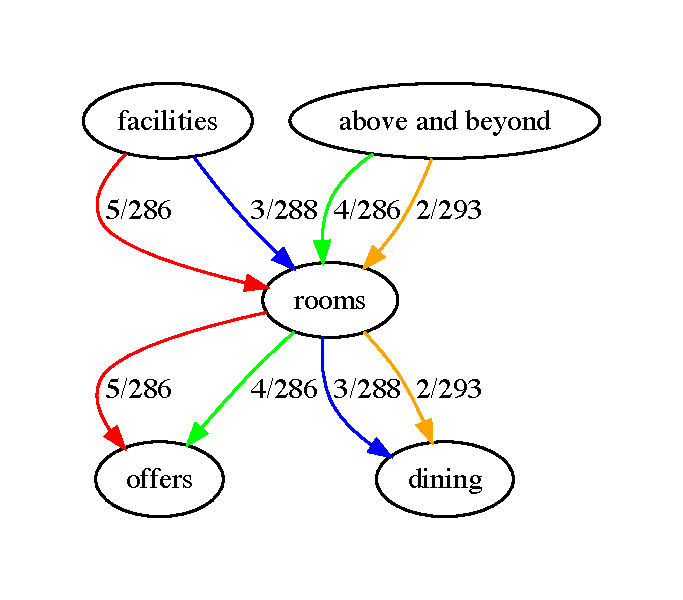
\includegraphics{figs/digraphs/sample_graph}
  \caption[Sample frequency patterns identified in a subset of PC requests]{Sample frequency patterns identified in a subset of PC requests. Refer to Table~\ref{tab:sample_graph} for frequency pattern interactions.}
  \label{fig:sample_graph}
\end{figure}